% Copyright 2004 by Till Tantau <tantau@users.sourceforge.net>.
%
% In principle, this file can be redistributed and/or modified under
% the terms of the GNU Public License, version 2.
%
% However, this file is supposed to be a template to be modified
% for your own needs. For this reason, if you use this file as a
% template and not specifically distribute it as part of a another
% package/program, I grant the extra permission to freely copy and
% modify this file as you see fit and even to delete this copyright
% notice. 

\documentclass{beamer}

% There are many different themes available for Beamer. A comprehensive
% list with examples is given here:
% http://deic.uab.es/~iblanes/beamer_gallery/index_by_theme.html
% You can uncomment the themes below if you would like to use a different
% one:
%\usetheme{AnnArbor}
%\usetheme{Antibes}
%\usetheme{Bergen}
%\usetheme{Berkeley}
%\usetheme{Berlin}
%\usetheme{Boadilla}
%\usetheme{boxes}
%\usetheme{CambridgeUS}
%\usetheme{Copenhagen}
%\usetheme{Darmstadt}
%\usetheme{default}
%\usetheme{Frankfurt}
%\usetheme{Goettingen}
%\usetheme{Hannover}
%\usetheme{Ilmenau}
%\usetheme{JuanLesPins}
%\usetheme{Luebeck}
\usetheme{Madrid}
%\usetheme{Malmoe}
%\usetheme{Marburg}
%\usetheme{Montpellier}
%\usetheme{PaloAlto}
%\usetheme{Pittsburgh}
%\usetheme{Rochester}
%\usetheme{Singapore}
%\usetheme{Szeged}
%\usetheme{Warsaw}

\usepackage{kotex}
\usepackage{braket}
\usepackage{array}
\usepackage{calc}
\usepackage{datetime}


\usepackage{listings}


\title{Programming Problems with Python  }

% A subtitle is optional and this may be deleted
\subtitle{Fastcampus Math Camp}

\author{신승우}
% - Give the names in the same order as the appear in the paper.
% - Use the \inst{?} command only if the authors have different
%   affiliation.

% \institute[Universities of Somewhere and Elsewhere] % (optional, but mostly needed)
% {
  % \inst{1}%
  % Department of Computer Science\\
  % University of Somewhere
  % \and
  % \inst{2}%
  % Department of Theoretical Philosophy\\
  % University of Elsewhere}
% - Use the \inst command only if there are several affiliations.
% - Keep it simple, no one is interested in your street address.

% - Either use conference name or its abbreviation.
% - Not really informative to the audience, more for people (including
%   yourself) who are reading the slides online

\subject{Theoretical Computer Science}

% This is only inserted into the PDF information catalog. Can be left
% out. 

% If you have a file called "university-logo-filename.xxx", where xxx
% is a graphic format that can be processed by latex or pdflatex,
% resp., then you can add a logo as follows:

% \pgfdeclareimage[height=0.5cm]{university-logo}{university-logo-filename}
% \logo{\pgfuseimage{university-logo}}

% Delete this, if you do not want the table of contents to pop up at
% the beginning of each subsection:


% Let's get started
\begin{document}

\begin{frame}
  \titlepage
\end{frame}






\begin{frame}[allowframebreaks]{비밀 지도} 
네오는 평소 프로도가 비상금을 숨겨놓는 장소를 알려줄 비밀지도를 손에 넣었다. 그런데 이 비밀지도는 숫자로 암호화되어 있어 위치를 확인하기 위해서는 암호를 해독해야 한다. 다행히 지도 암호를 해독할 방법을 적어놓은 메모도 함께 발견했다.

지도는 한 변의 길이가 n인 정사각형 배열 형태로, 각 칸은 “공백”(“ “) 또는 “벽”(“\#”) 두 종류로 이루어져 있다.
전체 지도는 두 장의 지도를 겹쳐서 얻을 수 있다. 각각 “지도 1”과 “지도 2”라고 하자. 지도 1 또는 지도 2 중 어느 하나라도 벽인 부분은 전체 지도에서도 벽이다. 지도 1과 지도 2에서 모두 공백인 부분은 전체 지도에서도 공백이다.
“지도 1”과 “지도 2”는 각각 정수 배열로 암호화되어 있다.
암호화된 배열은 지도의 각 가로줄에서 벽 부분을 1, 공백 부분을 0으로 부호화했을 때 얻어지는 이진수에 해당하는 값의 배열이다. 

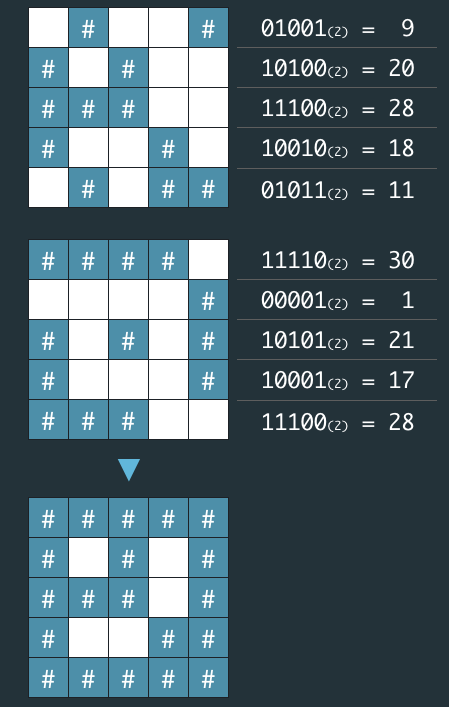
\includegraphics[height=5cm,keepaspectratio]{map}

\end{frame}


\begin{frame}[allowframebreaks]{다트 문제} 

카카오톡 게임별의 하반기 신규 서비스로 다트 게임을 출시하기로 했다. 다트 게임은 다트판에 다트를 세 차례 던져 그 점수의 합계로 실력을 겨루는 게임으로, 모두가 간단히 즐길 수 있다.
갓 입사한 무지는 코딩 실력을 인정받아 게임의 핵심 부분인 점수 계산 로직을 맡게 되었다. 다트 게임의 점수 계산 로직은 아래와 같다.
\begin{itemize}
\item 다트 게임은 총 3번의 기회로 구성된다.
\item 각 기회마다 얻을 수 있는 점수는 0점에서 10점까지이다.
\item 점수와 함께 Single(S), Double(D), Triple(T) 영역이 존재하고 각 영역 당첨 시 점수에서 1제곱, 2제곱, 3제곱으로 계산된다.
\item 옵션으로 스타상(*) , 아차상(\#)이 존재하며 스타상(*) 당첨 시 해당 점수와 바로 전에 얻은 점수를 각 2배로 만든다. 아차상(\#) 당첨 시 해당 점수는 마이너스된다.
\item 스타상(*)은 첫 번째 기회에서도 나올 수 있다. 이 경우 첫 번째 스타상(*)의 점수만 2배가 된다. 
\item 스타상(*)의 효과는 다른 스타상(*)의 효과와 중첩될 수 있다. 이 경우 중첩된 스타상(*) 점수는 4배가 된다. (예제 4번 참고)
\item 스타상(*)의 효과는 아차상(\#)의 효과와 중첩될 수 있다. 이 경우 중첩된 아차상(\#)의 점수는 -2배가 된다. (예제 5번 참고)
\item Single(S), Double(D), Triple(T)은 점수마다 하나씩 존재한다.
\item 스타상(*), 아차상(\#)은 점수마다 둘 중 하나만 존재할 수 있으며, 존재하지 않을 수도 있다.
\end{itemize}

0부터 10의 정수와 문자 S, D, T, *, \#로 구성된 문자열이 입력될 시 총점수를 반환하는 함수를 작성하라. 
\end{frame}


\begin{frame}{Huffman Coding (Optional)}
Huffman Coding은 무손실 압축의 대표적인 예제이다. 가장 많이 쓰이는 압축법 중 하나인데, 다음과 같은 순서로 이루어진다. 
\begin{itemize} 
\item 문자열들을 가장 많이 쓰이는 순서대로 배열한다. 
\item 가장 많이 쓰이는 문자에 0, 그 다음으로 많이 쓰이는 문자에 1, ... 과 같은 식으로 모든 문자에 이진수를 할당한다. 
\item 문자열을 할당된 이진수로 바꾼 후 리턴한다. 
\end{itemize}

주어진 문자열을 압축하고, 압축율을 계산하고, 다시 복원해서 원래 문자열과 같은 것을 보여라. 

\end{frame}


\begin{frame}[allowframebreaks]{블록 지우기 문제  (Optional)}

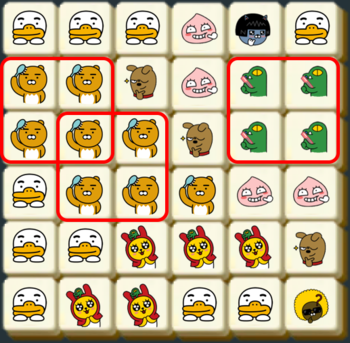
\includegraphics[width=5cm,keepaspectratio]{prob6} 

같은 블록이 2*2 형태로 붙어 있으면 사라지게 된다. 이 때, 주어진 첫 블록에서 몇 개가 사라지는지 구하라. 

\end{frame}


\begin{frame}{파일구조 다루기}

주어진 파일 디렉토리에서, 다음 일들을 하는 함수를 구현하라. 

\begin{itemize}
\item 주어진 확장자의 파일 다 출력하기. 확장자가 특정되지 않았으면 모든 파일 다 출력하기. 
\item 모든 폴더 다 출력하기. 
\end{itemize}


\end{frame}

\begin{frame}{정규표현식 예제} 
다음 항목들을 matching하는 정규표현식을 만들어라. 

\begin{itemize} 
\item 전화번호 
\item 이메일 (아이디는 알파벳과 숫자만 허용. 도메인은 ***.com 만 허용)
\end{itemize}

또, 파일 안에 있는 정규표현식에 맞는 문장을 하나 입력하라. 

%\begin{itemize} 
%\item \textasciicircum[1-9][0-9]*\textdollar
%\item \textasciicircum(19|20)\backslash d \backslash d[- /.](0[1-9]|1[012])[- /.](0[1-9]|[12][0-9]|3[01])\textdollar
%\end{itemize} 
\end{frame}

\begin{frame}[allowframebreaks]{크롤러} 

네이버 웹툰의 제목을 크롤링해 보자. 링크는 http://comic.naver.com/webtoon/weekday.nhn 를 이용하라. 

\end{frame}

% \subsection{Primitive Data Types and Supported Methods} 

% \begin{frame}{String}
% \begin{itemize}
% \item count()
% \item endswith()
% \item find()
% \item split() 
% \item strip()
% \end{itemize}

% \end{frame}

% \begin{frame}{List/Tuple}
% \begin{itemize}
% \item append()
% \end{itemize}

% \end{frame}

% \begin{frame}{dict}
% \begin{itemize}
% \item 
% \end{itemize}

% \end{frame}


% \subsection{Defining Functions} 
% % def/lambda
% \subsection{Frequently Used Functions} 
% % 
% \subsection{File I/O}

% \section{Python as an Object-Oriented Language} 

% \subsection{Defining Classes} 

% \subsection{Class Magic Methods} 

% \subsection{Class Inheritance} 

% \subsection{\_\_dict\_\_ and setattr Function} 


% % \section{Python as a Functional Lanuguage} 

% % \subsection{What is being Functional?} 

% % \subsection{$\lambda$-expression} 

% % \subsection{Map, Reduce, Filter} 

% \section{Topics on Python} 

% \subsection{Generator vs Iterator vs Iterable} 

% \subsection{Builtin Functions}

% % \subsection{Recursion}

% \section{Understanding Python Code}

% \subsection{Interpreters as Subsititution}

% \subsection{Namespaces and local()} 

% \subsection{Python Namespaces}

% \subsection{How is Python Namespace Constructed?}


% \section{Python Style Guide}

% \section{Useful Libraries} 

% \subsection{os}

% \subsection{re} 

% \subsection{BeautifulSoup/Request} 



% \section{"Maybe" Useful Libraries} 

% \subsection{Inspect} 

% \subsection{PyMonad}

\end{document}


